\chapter{Introducción}\label{chap:introduccion}
%Motivation

En los últimos años, con el crecimiento de plataformas online como Amazon, Netflix, YouTube y muchas otras, los contenidos disponibles para los usuarios han crecido de forma exponencial, habiéndose tripicado el número de películas lanzadas desde el año 2000 \cite{watson_2020} y multiplicado por 100 el número de horas subidas a YouTube cada minuto \cite{clement_2019}. \\

Hace no mucho tiempo si uno tenía que comprar un pequeño electrodoméstico para la cocina iba a una tienda especializada en ello. Si quería ver una película iba aun videoclub donde se le podían recomendar películas y alquilarlas, etc. Sin embargo, con el auge de Internet han aparecido plataformas que integran muchos de estos servicios. Amazon es un terrible centro comercial en el que podemos encontrar desde alimentación hasta arte, pasando por tecnología, libros... e incluso ver películas en su plataforma. YouTube, por su parte, es una plataforma en la que los propios creadores de contenido suben de forma diaria $26$ millones de horas de vídeo al día y $1000$ millones de horas son visualizadas cada día por sus $2000$ millones de usuarios \cite{YoutubeStats}. Queda a la vista el hecho de que en los últimos años ha tenido lugar un cambio en el orden de magnitud de las plataformas de venta, pasando de pequeñas tiendas o cadenas nacionales a plataformas internacionales.\\

Uno de los grandes retos que estas plataformas han tenido que abordar es mantener a sus usuarios en ellas. Pongamos por ejemplo una persona en un ordenador con los miles de millones de vídeos que hay en YouTube, o delante de todos los contenidos que hay disponibles para visualizar en Netflix (1770 títulos en España \cite{Lovely2019}). El elegir qué contenido consumir puede ser una tarea de tal magnitud, que consiga ahuyentar al usuario. Por tanto, parece que ya no es suficiente con tener en la plataforma (tienda, antes; web, ahora) contenidos atractivos para el usuario, ni siquiera es ya suficiente con conseguir los usuarios acceder a la plataforma en cuestión dispuestos a usarla, sino que es vital que sea la plataforma quien les ayude a filtrar el contenido que puede ser de su agrado.\\

Por su parte, los hábitos de consumo de los usuarios también han evolucionado mucho en los últimos años. Desde escuchar la opinión de un producto de uno o varios vendedores y de su círculo más cercano hasta contar en la actualidad con grandes redes de encuentro entre usuarios donde diferentes productos son valorados y analizados. En un ejemplo concreto, una persona que quiera comprar un equipo de música para su hogar, hace unos años hubiera ido a una tienda cercana a su casa, hubiera preguntado al vendedor y, en base a la opinión del mismo y su presupuesto, hubiera realizado una elección. En la actualidad, podría buscar equipos de música en Amazon, que le serían ordenados según opiniones de otros usuarios, hubiera podido leer cientos de opiniones personales de compradores, visto análisis de expertos en YouTube, que analizarían de forma más objetiva las ventajas e inconvenientes de cada producto.\\

Se puede decir que con la llegada de estas plataformas ha llegado también la necesidad de ser capaz de orientar al consumidor dentro de las mismas, ya que de no hacerlo existe el riesgo de que el usuario se vea abrumado y no sea capaz de utilizarla. Tampoco puede decirse que el beneficio de ser capaz de realizar una recomendación al usuario sea sólo para él. La forma que tiene YouTube de recomendarte vídeos puede hacer que lo que iba a ser una visita de $10$ minutos se transforme en media tarde viendo vídeos y, en consecuencia, anuncios.\\

Nuestras intenciones y las de las plataformas online, no tienen por qué estar alineadas. Las plataformas actuales tienen motores de recomendación potentes, capaces de mantener a sus usuarios en la plataforma. Sin embargo, muchos los usuarios lo que desean es tratar de ver el contenido que mas les pueda gustar, independientemente de la plataforma en la que se encuentre. Las compañías usan un acercamiento que tiene en cuenta primero la plataforma, ya que recomiendan contenido que ellos tienen disponible. Mientras tanto, muchos usuarios pueden preferir un acercamiento que dé prioridad al contenido, sin importar la plataforma.

Ha quedado patente que en la actualidad se hace necesario disponer de sistemas que en base al contenido disponible y la opinión de los distintos usuarios sean capaces de recomendar productos de la plataforma \cite{Konstan2004}. La intención del proyecto es desarrollar un motor de recomendación que, sin disponer de la misma cantidad de datos que plataformas como Netflix, sea capaz de obtener unos resultados de satisfacción comparables, pero sin tener en cuenta la plataforma de visionado del contenido.


%%%           %%%
%  Objectives   %
%%%           %%%
\section{Objetivos del proyecto}\label{sec:objetivos}

Como se ha visto anteriormente, es muy beneficioso para las empresas que ofrecen productos online ser capaces de recomendar a sus usuarios otros productos a partir de los ya consumidos. Esto tiene, dos ventajas fundamentales:

\begin{itemize}
    \item La plataforma es capaz de orientar al usuario, de forma que se evita una posible fuga de usuarios a otras plataformas ante la ingente cantidad de productos a consumir.
    \item Una vez el usuario ha consumido un producto pueden serle recomendados otros relacionados, incrementando el número de productos consumidos por el usuario.
\end{itemize}

En este trabajo utilizaremos un conjunto de datos compuesto por información sobre películas, con la finalidad de construir un sistema de recomendación de películas que, partiendo de una película propuesta por el usuario, pueda recomendarle otras similares. La diferencia con el motor de búsqueda de plataformas como Netflix, es que estará disponible fuera de estas plataformas, en una app tan común como Telegram, y que recomendará películas de todo tipo, no solo las que estén en una determinada plataforma. ¿Es posible crear un sistema de recomendación usando recomendación basada en contenido? ¿Es Telegram una buena vía para realizar esta recomendación? ¿Prefiere el usuario recomendaciones que no tengan en cuenta la plataforma, pudiendo ver contenido más variado? Estas son algunas de las preguntas que trataremos de resolver en este proyecto. La forma en la que tratremos de mejorar los sistemas de plataformas como Netflix o Prime Video será, por tanto, en términos de riqueza del contenido y de posibilidad de recibir recomendaciones en cualquier situación, no solo dentro de estas plataformas.\\

El conjunto de datos utilizado posee metadatos sobre las películas, como palabras clave, presupuesto, puntuación de los usuarios... Información relevante y suficiente para poder implementar este sistema. Como puede deducirse, es necesario un soporte para este sistema que permita al usuario final poderlo utilizar. Lo habitual sería integrarlo con un trabajo de User Experience (UI) y que quedara, por tanto, integrado en la plataforma. En este caso no disponemos de una plataforma en la que integrar el sistema, por lo que se creará una API (que contendrá el sistema de recomendación) que podrá ser llamada por un bot de Telegram, de forma que recomiende películas a un usuario a partir de otra.\\

\begin{figure}[h]
    \centering
    \captionsetup{width=10cm}
    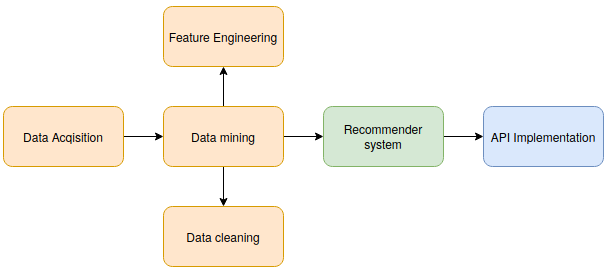
\includegraphics[width=12cm]{contenido/imagenes/initial.png}
    \caption{Proceso de tratado de la información para la creación del sistema de recomendación.}
    \label{fig:process}
\end{figure}

El proceso que se seguirá para la creación del sistema de recomendación se muestra en la \autoref{fig:process} y consistirá de los siguientes pasos:
\begin{enumerate}
    \item Adquisición de los datos y limpieza de los mismos.
    %\item Análisis preliminar avanzado de los datos.
    \item Creación del sistema de recomendación.
    \item Creación de la API e integración en el bot de Telegram.
\end{enumerate}


%%%                  %%%
% Document structure   %
%%%                  %%%
\section{Estructura de la memoria}\label{sec:estructura}

El trabajo, como se ha descrito en los capítulos anteriores, tiene como objetivo la creación de un sistema de recomendación de películas, aunque se tratará de incluir en el mismo el flujo \textit{end to end} de tratamiento de la información. El trabajo se estructurará en diferentes capítulos, conteniendo cada uno de ellos una de las partes del flujo. Los capítulos que se incluirán en este trabajo serán los siguientes:

\begin{itemize}
    \item \autoref{chap:adq}: Estructura de los datos a utilizar y preprocesado de los mismos. En este capítulo se realizará una presentación y explicación de los datos de los que se dispone, de forma que se entiendan los siguientes pasos seguidos.
    %\item \textit{Preliminary Data Analysis}. Caso de uso de análisis de datos para resolución de preguntas de negocio. %Al trabajar con un conjunto de datos siempre es importante realizar un análisis previo, de forma que pueda %entenderse la estructura de los mismos. También se verá la utilidad de disponer de un conjunto de datos %relativamente grande a la hora de responder a preguntas que pueden surgir en relación con la informacion contenida %en los mismos.
    \item \autoref{chap:recom}: Sistemas de recomendación. Se realizará una explicación de la teoría que existe tras estos sistemas y los diferentes tipos que existen. Se creará el sistema de recomendación.
    \item \autoref{chap:api}: Integración del sistema en una API y creación de un chatbot. Es importante que nuestro sistema de recomendación sea explotable por los usuarios, de nada sirve tener un buen sistema de recomendación si no puede ser usado. Se explicará la creación de un bot de Telegram y cómo crear una API que pueda ser llamada por el bot.
    \item \autoref{chap:resultados}: Próximos pasos. Finalmente, se realizará un repaso de lo desarrollado en el trabajo y se propondrán puntos en los que mejorar el sistema que no hayan podido implementarse por algún motivo.
\end{itemize}

\section{Trabajo desarrollado}\label{sec:trabajodesarrollado}

En esta memoria, se trata de solventar el problema que se ha comentado en las secciones anteriores. Las plataformas de contenido disponen de sistemas de recomendación potentes, pero con una limitación de origen: solo recomiendan contenido de sus plataformas. Esto hace que si vemos una película concreta en una plataforma y esta nos recomienda otra, es posible que haya mejores recomendaciones que la plataforma en cuestión no esté realizando debido a que no dispone de ese contenido. 

Tal y como se verá en el \autoref{chap:recom}, un tipo de motores de recomendación son los motores basados en contenido. Estos motores se basan en características intrínsecas de las películas y no tanto en las opiniones atómicas de los usuarios. En la solución propuesta en este trabajo, las palabras clave que describen una película son la parte central de la recomendación. Esta elección se ha realizado principalmente por los datos disponibles, ya que los temas de una película, su año de producción o la opinión media de los usuarios son datos relativamente abiertos, mientras que las opiniones concretas de cada usuario son algo propiedad de las plataformas en las que se realizan estas valoraciones, por lo que no tenemos acceso a estos datos. 

Para realizar la recomendación y una vez se ha limpiado el dataset, las películas se distribuyen en un espacio vectorial de keywords y se seleccionan en base a una distancia las más próximas a la película dada. Una vez se tienen las películas más cercanas a la película dada, se establece una heurística que puntúa cada una de estas películas en función de su puntuación, su año de producción y el ratio entre votos e ingresos. Esta heurística trata de, una vez se han seleccionado las películas candidatas a ser recomendadas, tratar de escoger de entre ellas las que probablemente prefiera el usuario. Por ejemplo, creemos que si tras ver una película de Harry Potter se nos recomienda una de magia similar pero del año 1950 es probable que el usuario sea reacio a escogerla.

Una de las principales ventajas de nuestro motor de recomendación, es la forma en la que se ha implementado. Al ser un motor agnóstico en términos de plataforma (ya que simplemente tiene datos de las películas y su puntuación en IMDB), necesitábamos un sitio desde el que pudiera ser explotado. De entre todos los posibles, hemos elegido implementarlo en un bot de Telegram, ya que Telegram es una plataforma con una gran expansión y además multiplataforma. Consideramos que la mayoría de usuarios tendrán a mano un dispositivo móvil cuando estén viendo películas, por lo que en cualquier momento pueden escribir un título al bot y éste les enviará las recomendaciones obtenidas.

Además, nuestro motor (y en general los motores basados en contenido) tiene una ventaja principal, y es que puede ser actualizado fácilmente con la llegada de nuevas películas a la cartelera. Dado que la información principal que utilizamos son las palabras clave, no necesitamos que un gran número de usuarios haya visto la película en cuestión para que tengamos la información suficiente para recomendar esa nueva película. Esto hace que sea un modelo especialmente beneficioso para que los usuarios puedan descubrir películas menos conocidas que puedan ser de su agrado.



    
